\section{Microcontroller-ul folosit}
Așa cum s-a menționat anterior, în cadrul acestei lucrări s-a optat pentru folosirea unui microcontroller pe 32 biți STM32F411 produs de compania ST Electronics, datorită capabilităților hardware oferite de acesta (modul USB integrat, posibilitatea de reducere a consumului de energie etc) și a suportului oferit de către companie sub forma documentației și programelor de dezvoltare (programare si configurare cipuri). În cele ce urmează vom detalia întregul raționament din spatele acestei alegeri.

\subsection{Oferta valabilă de microcontroller-e}
Ca parte a efortului derulat de cercetare și dezvoltare a acestui proiect au fost luate in considerare diferite microcontroller-e pentru a satisface obiectivele propuse. Pentru a face o decizie evident va fie nevoie să stabilim niște criterii obiective. Astfel microcontroller-ul ales va trebui să satisfacă următoarele condiții:

\begin{enumerate}
	\item Microcontroller-ul ales va trebui să faciliteze comunicația cu calculatorul utilizatorului prin portul USB.
	\item Microcontroller-ul ales va trebui să ofere facilități de depanare fără a fi nevoiți să afișăm pe ecran starea acestuia la un moment dat.
	\item Microcontroller-ul ales va trebui să fie acompaniat de un toolchain pentru a facilita procesul de dezvoltare a proiectului.
	\item Microcontroller-ul ales va trebui să ofere programatorului cel puțin două interfețe de I2C (motiv care va fi înțeles când vom prezenta protocolul intern de comunicație al ceasului DGT3000).
\end{enumerate}

Acestea fiind enunțate este momentul să discutăm despre cele mai populare opțiuni disponibile pe piață.
\begin{enumerate}
	\item ATmega328p
	\item ESP8266
	\item STM32F411
\end{enumerate}

\paragraph{ATmega328p} oferit de către Atmel (Microchip acum) este un microcontroller pe 8 biți bazat pe arhitectura AVR, fiind foarte popular printre amatori datorită includerii sale in familia de plăci Arduino. Popularitatea este justificată prin complexitatea redusă a acestuia și a resurselor online disponibile (fie că discutăm de programarea bare-metal sau folosind framework-ul Arduino \cite{arduino_docs}) iar toolchain-ul format din avr-libc (implementarea AVR a standardului C), avr-gcc (driver-ul folosit pentru compilare) și avr-dude (utilitar folosit pentru încărcarea fișierelor binare) este ușor de procurat și integrat în cadrul proiectelor. Așadar putem considera din start cel de al treilea criteriu drept satisfăcut. Referitor la primele două, acestea sunt problematice.
Dacă ar fi să privim fișa de catalog a acestui microcontroller se va putea observa că acesta nu oferă facilitatea de a comunica folosind protocolul USB \cite{atmega_datasheet}, așa că cei de la Arduino au inclus în plăcile lor un cip cu rolul de a converti datele transmise prin UART (Universal Asynchronous Receiver Transmitter; protocol disponibil pe Atmega328p) în USB. Intr-adevăr, dacă privim schema electrică unde datele din conectorul USB sunt transmise către acest cip, iar dacă căutam pe pagina oficială a acestora regăsim următoarea informație în secțiunea \textit{Communication}:
\begin{quote}
The ATmega328 provides UART TTL (5V) serial communication, which is available on digital pins 0 (RX) and 1 (TX). An ATmega16U2 on the board channels this serial communication over USB and appears as a virtual com port to software on the computer \cite{arduino_usb}.
\end{quote}
\textbf{NOTĂ:} multe plăci fiind clone ale originalului folosesc în loc de ATmega16U2 un alt convertor, și anume CH340. \\
Trecând la următorul criteriu (facilitatea de depanare a programelor), acesta este încălcat și ne obligă să considerăm alte opțiuni. În ciuda faptului că documentația oficială \cite{atmega_datasheet} specifică un sistem de depanare pe cip (debugWIRE), problema rămâne de interfațarea cu acesta. Plaăcile Arduino nu oferă o soluție iar procurarea unor programatoare pentru acest protocol este dificilă din cauza indisponibilității sau a prețului acestora. Dacă este să abordăm chestiunea interfețelor I2C din nou ne lovim de o problemă deoarece acest microcontroller dispune doar de un singur canal fizic (numit oficial în documentație \textbf{Two-Wire Interface}).

\paragraph{ESP8266} de la Espressif reprezintă un System on a Chip (SoC) popular de asemenea printre amatori datorită costului său redus, integrării cu tehnologie Wi-Fi (utilă pentru implementarea soluțiilor ce țin de Internet of Things) și a tool-urilor existente. De cele mai multe ori se poate opta pentru a programa cipul în limbajul LUA (abstractizând și mai mult interacțiunea hardware) iar proiectele sunt ușor de integrat în Arduino IDE sau PlatformIO. Din nou, cel de al treilea criteriu este satisfăcut. Similar cu cu ATmega328p, acest SoC nu prezintă o interfață USB\cite{esp_tech}, fiind din nou nevoie de a se folosi un convertor (a se vedea de exemplu NodeMCU). Trecând la penultimul criteriu, ESP8266 nu prezintă de nici un fel un protocol de depanare, singura soluție practică fiind a ocupa portul serial cu scrierea pe ecran, ceea ce nu ne convine (ideal am dori să folosm acest port doar pentru a transmite sau citi date de la PC spre MCU). Aruncându-ne privirea spre ultimul criteriu observăm ca nici acesta nu este satisfăcut deoarece integratul de față oferă doar o singură interfață fizică pe care o putem folosi.

\paragraph{STM32F411} oferit de compania ST Electronics este un microcontroller pe 32 de biți care satisface toate cele trei criterii. Acesta se bucură de documentație excelentă de către furnizor și comunitate, este însoțit de un toolchain flexibil (care va fi prezentat în cele ce urmează), are modul de USB deja integrat și, cel mai important, oferă programatorului facilitatea de depanare pe cip prin uzul protocoalelor Serial Wire Debug și JTAG. Așadar, considerăm acest microcontroller alegerea cea mai bună pentru scopul propus, iar drept placă s-a optat pentru folosirea WeAct BlackPill v2.0. A nu se uita nici faptul că aceste MCU prezintă programatorului nu două ci chiar trei canale fizice de I2C pentru a fi folosite (ne vom mulțumi cu două în cele ce va urma).

\subsection{Ecosistemul STM32}
Unul dintre motivele pentru care cipurile din familia STM32 sunt atît de răspîndite îl constituie ecosistemul bogat de tool-uri pe care ST le-a pus la dispoziția utilizatorilor. Succint le vom prezenta.
\paragraph{STM32CubeMX}
Cu căt tehnologia avansează și cât mai multe funcționalități sunt integrate in siliciu automat crește și în complexitate programarea acestuia. Dacă pentru vechiul ATmega328p ajungeau setarea a câtorva regiștrii pentru a obține configurația dorită, la microcontroller-ele noi cum ar fi cele de la ST sau NXP aceasta nu mai este o sarcină facilă. Norocul nostru este că ST oferă programatorilor o aplicație cu o interfață grafică simplă și intuitivă ce permite configurarea cipului, generând apoi cod automat pentru aceasta. Pentru implementarea soluției noastre acest generator a fost cu mult benefic.

\paragraph{STM32CubeIDE}
Perifericele fiind configurate se pune problema de a dezvolta aplicația în sine, indiferent de nivelul de complexitate a acesteia. Aici intervine STM32Cube Integrated Development Environment ce prezintă utilizatorului un editor grafic de text (bazat pe tehnologia Eclipse), sistem de gestionare a proiectelor in format XML, toolchain complet de compilare (vorbim aici de programe precum driver-ul GCC) și integrare cu server GDB de depanare (evident fiind nevoie de un programator conectat la PC). Cei care nu doresc a folosi acest editor îl pot integra ca extensie in  Visual Studio Code sau dacă chiar se dorește, orice editor de text combinat cu un \textit{build system} cum ar fi Make sau CMake.

\paragraph{STM32CubeProgrammer}
Ajungând in punctul în care fișierul în format binar al aplicației este generat, se pune problema încărcării acestuia pe microconstroller. O modalitate facil[] de a indeplini aceasta o reprezintă STM32CubeProgrammer ce poate detecta automat programatoarele conectate la PC, încărca codul și inspecta locațiile de memorie.

\paragraph{Surse de informații}
Evident că pentru orice proiect în curs de dezvoltare sursa principală de informații va trebui să fie formată din \textit{datasheet-ul} și \textit{reference manual-ul} aferente microcontroller-ului ales. Clar cei de la ST ne pun la dispoziția noastra aceste documente plus manuale pentru aplicații practice cum ar fi citirea și procesarea semnalelor analogice, însă spre norocul nostru avem parte si de o bibliografie online întreținută de comunitate \footnote{A se consulta următorul link: \url{https://stm32world.com/wiki/Main_Page}}. 

\subsection{Placa de dezvoltare folosită}
Așa cum s-a argumentat anterior, pentru dezvoltarea acestei lucrări de licență s-a ales micrcontroller-ul STM32F411. Acesta are la bază un nucleu ARM Cortex-M4 (profilul M este cel mai adesea folosit pentru aplicatții ce impun un consum redus de energie), interfețe dedicate pentru programare și depanare (protocoalele Serial Wire Debug și JTAG), canale pentru comunicație serială cum ar fi I2C, USB și multe alte facilități care vor fi evidențiate în aplicații mai complexe decât cea a temei de față. Nu trebuie să ne lasăm intimidați de diagrama bloc a MCU-ului atașată mai jos, chiar dacă este la prima vedere se se observă o multitudine de module.
\begin{figure}[H]
	\centering
	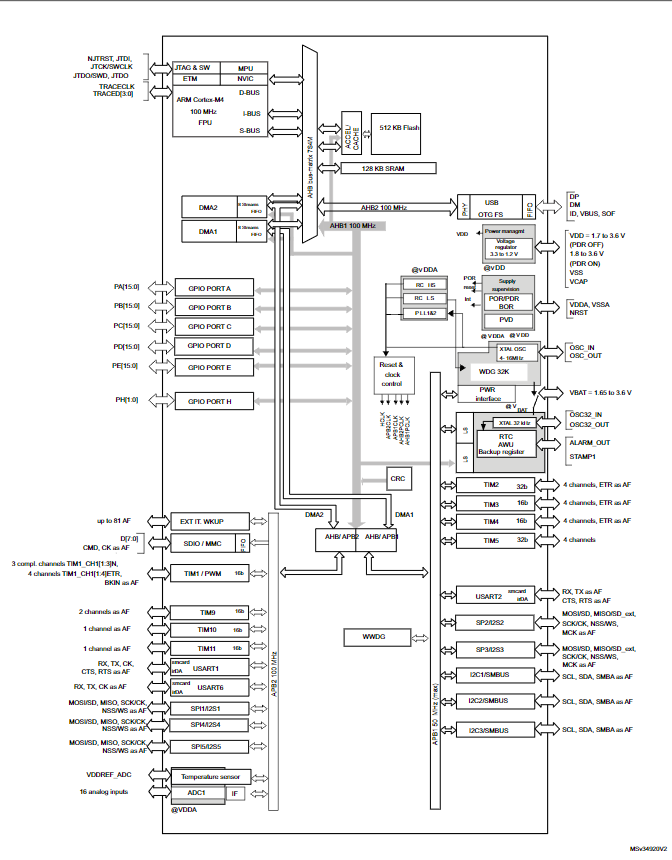
\includegraphics[width=0.7\textwidth]{img/stm32_block.png}
	\caption{STM32F411 schemă bloc}
\end{figure}

Modelând acest sistem de calcul după arhitectura Von Neumann observăm imediat că acesta dispune de cele trei subasamble fundamentale și anume:
\begin{enumerate}
	\item Unitatea de calcul: subsistem usor de observat, este reprezentat de blocul ce conține nucleul Cortex-M4 în sine, controller-ul de întreruperi (Nested Vector Interrupt Controller; NVIC), unitate de protecție a memoriei de program (Memory Protection Unit; MPU), și o unitate pentru calculul valorilor în virgulă mobilă (Floating Point Unit; FPU)
	\item Modulele de intrare-ieșire: se referă la blocurile care sunt \textit{periferice} unității de calcul și care presupun îndeplinirea unor funcționalități specifice și posibilitatea de configurare a acestora. Amintim aici de module precum pinii de uz general (GPIO), interfețele I2C și temporizatoarele.
	\item Magistrala: în cazul de față observăm standardul ARM AMBA care este împarțită în liniile AHB (Advanced High Performance Bus) și APB (Advanced Peripheral Bus).
\end{enumerate}

Rareori în zilele de azi se mai programează direct pe microcontroller deoarece deseori acesta necesită un circuit de alimentare și stabilizare a tensiunii, oscilator pentru configurarea temporizatoarelor ș.a.m.d. . Așa că, se optează pentru integrarea acestora într-un circuit imprimat pentru a facilita programarea acestuia (și eventual oferirea de componente cu scop de testare cum ar fi butoane sau LED-uri), deseori acestă abordare fiind numită placă de dezvoltare. Pentru lucrarea de față s-a optat pentru folosirea plăcii WeAct Studio Black Pill v2, găsit pe piață la un preț rentabil și asamblată într-un pachet de compactă. Spre avantajul nostru regăsim un oscilator de 25 MHz ce va fi folosit pentru configurarea ceasului perifericului USB.
\begin{figure}[H]
	\centering
	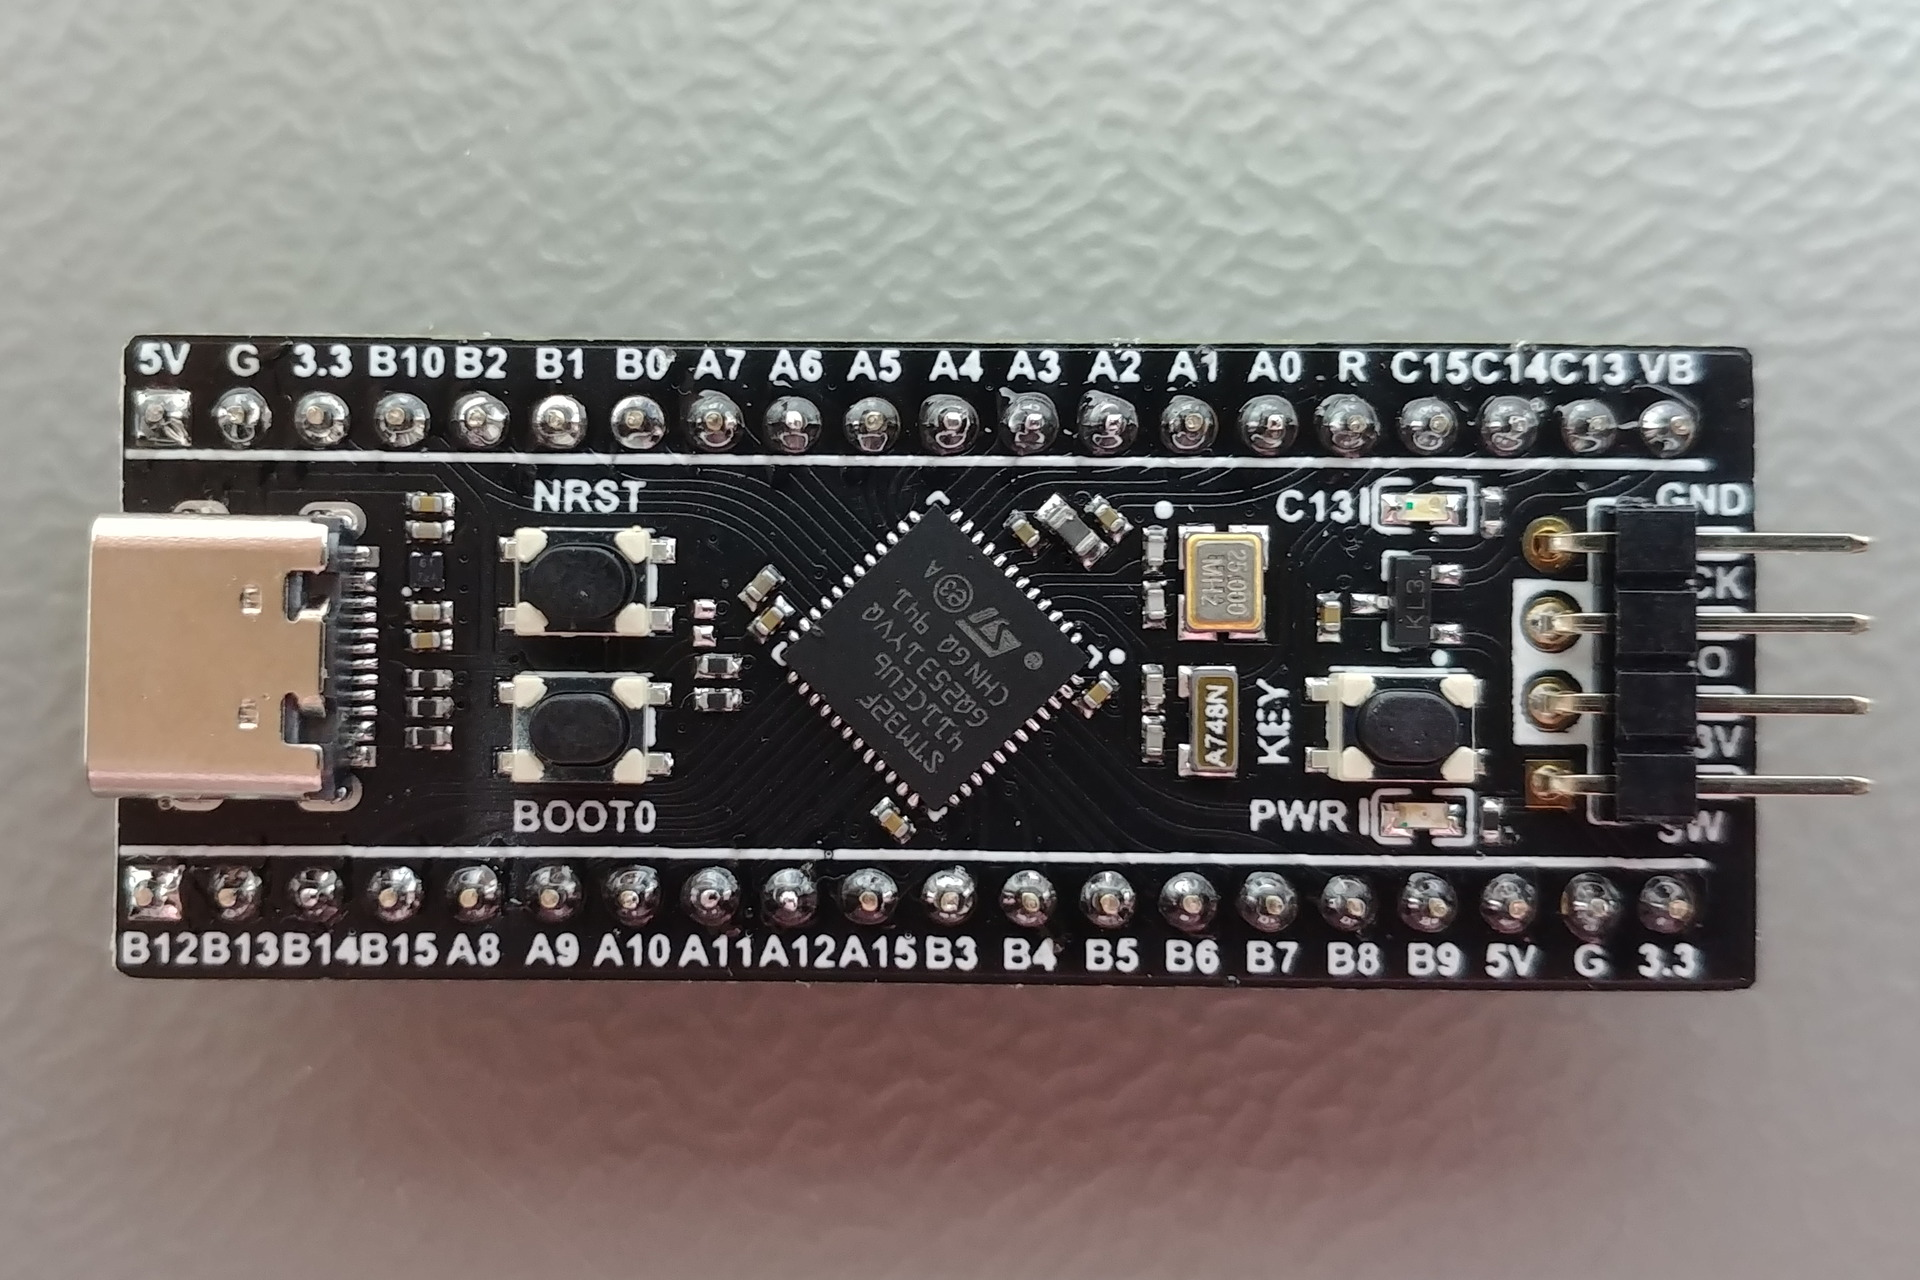
\includegraphics[width=0.7\textwidth]{img/blackpill.jpg}
	\caption{Placa WeAct Studio v2 Black Pill}
\end{figure}